% One-page executive tear sheet.
\documentclass[11pt,a4paper]{article}
\usepackage[top=13mm,bottom=15mm,left=16mm,right=16mm,footskip=6.5mm]{geometry}
\usepackage{style/quantedge}
% Generated by scripts/generate_report_data.py from the verified reference. Do not edit.

\newcommand{\qeBundle}{1c7bd6007fe22b014b25}
\newcommand{\qeDataset}{qe1\_20050101\_20261030\_r3\_6c4633a7ba}
\newcommand{\qeConfigHash}{587ddbe363589fb6956c23c5fe8b2b544bac81d9224a0b4bb59f60f5fbc0a017}
\newcommand{\qeProtocolCommitOriginal}{782ec20}
\newcommand{\qeProtocolCommit}{16181c0}
\newcommand{\qeHurdle}{6.75\%}
\newcommand{\qeSpending}{4.00\%}
\newcommand{\qeInflation}{2.50\%}
\newcommand{\qeFee}{0.25\%}
\newcommand{\qeRealGrowth}{0.00\%}
\newcommand{\qeHorizon}{10}
\newcommand{\qeBudgetVarNinetyFive}{1.00\%}
\newcommand{\qeBudgetVar}{1.50\%}
\newcommand{\qeBudgetEs}{2.00\%}
\newcommand{\qeBudgetVol}{10.00\%}
\newcommand{\qeBudgetDrawdown}{20.00\%}
\newcommand{\qeBudgetScenario}{20.00\%}
\newcommand{\qeBudgetVarUsd}{\$150,000}
\newcommand{\qeBudgetEsUsd}{\$200,000}
\newcommand{\qeBudgetDrawdownUsd}{\$2,000,000}
\newcommand{\qeDevCagr}{6.65\%}
\newcommand{\qeDevVol}{8.77\%}
\newcommand{\qeDevDrawdown}{−22.18\%}
\newcommand{\qeDevSharpe}{0.70}
\newcommand{\qeSelCagr}{10.38\%}
\newcommand{\qeSelVol}{7.74\%}
\newcommand{\qeSelDrawdown}{−14.47\%}
\newcommand{\qeSelSharpe}{1.14}
\newcommand{\qeEvalCagr}{7.63\%}
\newcommand{\qeEvalVol}{8.80\%}
\newcommand{\qeEvalDrawdown}{−16.78\%}
\newcommand{\qeEvalSharpe}{0.51}
\newcommand{\qeFullCagr}{7.68\%}
\newcommand{\qeFullVol}{8.58\%}
\newcommand{\qeFullDrawdown}{−22.18\%}
\newcommand{\qeFullSharpe}{0.72}
\newcommand{\qeEvalCagrSixty}{8.41\%}
\newcommand{\qeEvalVolSixty}{10.66\%}
\newcommand{\qeEvalDrawdownSixty}{−20.77\%}
\newcommand{\qeEvalSharpeSixty}{0.50}
\newcommand{\qeEvalCagrEqual}{13.69\%}
\newcommand{\qeFullBeta}{0.29}
\newcommand{\qeFullAlpha}{3.13\%}
\newcommand{\qeEvalAlpha}{0.77\%}
\newcommand{\qeHurdleGapDev}{−0.10\%}
\newcommand{\qeIncomeYield}{2.19\%}
\newcommand{\qeIncomeMean}{1.80\%}
\newcommand{\qeRealReturn}{4.88\%}
\newcommand{\qeCpiInflation}{2.59\%}
\newcommand{\qeSharpeAccrual}{0.719}
\newcommand{\qeSharpePrimary}{0.723}
\newcommand{\qeVar}{1.54\%}
\newcommand{\qeEs}{2.03\%}
\newcommand{\qeVarUsd}{\$153,950}
\newcommand{\qeEsUsd}{\$203,169}
\newcommand{\qeVarExcess}{\$3,950}
\newcommand{\qeEsExcess}{\$3,169}
\newcommand{\qeVarNinetyFive}{0.87\%}
\newcommand{\qeNormalVarNinetyFive}{0.90\%}
\newcommand{\qeFullVar}{1.63\%}
\newcommand{\qeFullEs}{2.50\%}
\newcommand{\qeFullEsUsd}{\$250,185}
\newcommand{\qeNormalVar}{1.29\%}
\newcommand{\qeNormalEs}{1.49\%}
\newcommand{\qeMcVar}{1.28\%}
\newcommand{\qePotEs}{2.03\%}
\newcommand{\qePotVar}{1.56\%}
\newcommand{\qeFullPotEs}{2.50\%}
\newcommand{\qeMcDraws}{25,000}
\newcommand{\qeHsFullExceptions}{65}
\newcommand{\qeFullSessions}{4,987}
\newcommand{\qeHsFullUc}{0.040}
\newcommand{\qeHsFullInd}{$1.7\times10^{-5}$}
\newcommand{\qeHsEvalUc}{0.394}
\newcommand{\qeHsEvalInd}{0.216}
\newcommand{\qeHsEvalExceptions}{18}
\newcommand{\qeNormalEvalExceptions}{27}
\newcommand{\qeNormalEvalUc}{0.004}
\newcommand{\qeEvalSessions}{1,464}
\newcommand{\qeBaselHs}{4}
\newcommand{\qeBaselNormal}{9}
\newcommand{\qeBaselHsZone}{green}
\newcommand{\qeBaselNormalZone}{yellow}
\newcommand{\qeBaselStart}{3 Nov 2025}
\newcommand{\qeBaselEnd}{30 Oct 2026}
\newcommand{\qeBaselExpected}{2.5}
\newcommand{\qeWeightSpy}{20.4\%}
\newcommand{\qeShareSpy}{29.6\%}
\newcommand{\qeWeightAgg}{40.0\%}
\newcommand{\qeShareAgg}{7.0\%}
\newcommand{\qeWeightGld}{25.0\%}
\newcommand{\qeShareGld}{31.6\%}
\newcommand{\qeWeightXle}{14.6\%}
\newcommand{\qeShareXle}{31.8\%}
\newcommand{\qeDivWeighted}{3.30\%}
\newcommand{\qeDivWeightedUsd}{\$329,643}
\newcommand{\qeDivBenefit}{38\%}
\newcommand{\qeCorrSpyAgg}{0.00}
\newcommand{\qeCorrSpyGld}{0.07}
\newcommand{\qeCorrSpyXle}{0.70}
\newcommand{\qeDriftSessions}{2,771}
\newcommand{\qeActiveSessions}{4,987}
\newcommand{\qeDriftMax}{45.14\%}
\newcommand{\qeDriftTicker}{AGG}
\newcommand{\qeDriftDate}{23 Oct 2008}
\newcommand{\qeDriftEquity}{37.30\%}
\newcommand{\qeGfcReturn}{−8.93\%}
\newcommand{\qeGfcDrawdown}{−23.87\%}
\newcommand{\qeGfcUsd}{\$892,991}
\newcommand{\qeGfcReturnSixty}{−29.99\%}
\newcommand{\qeGfcDrawdownSixty}{−30.33\%}
\newcommand{\qeCovidReturn}{−16.23\%}
\newcommand{\qeCovidDrawdown}{−18.84\%}
\newcommand{\qeCovidUsd}{\$1,622,750}
\newcommand{\qeCovidReturnSixty}{−20.59\%}
\newcommand{\qeCovidDrawdownSixty}{−20.81\%}
\newcommand{\qeRatesReturn}{−6.57\%}
\newcommand{\qeRatesDrawdown}{−13.36\%}
\newcommand{\qeRatesUsd}{\$656,660}
\newcommand{\qeRatesReturnSixty}{−20.58\%}
\newcommand{\qeRatesDrawdownSixty}{−20.63\%}
\newcommand{\qeHypoReturn}{−4.48\%}
\newcommand{\qeHypoDrawdown}{−4.48\%}
\newcommand{\qeHypoUsd}{\$447,652}
\newcommand{\qeHypoReturnSixty}{−19.80\%}
\newcommand{\qeHypoDrawdownSixty}{−19.80\%}
\newcommand{\qeFlags}{307}
\newcommand{\qeFlagNegative}{188}
\newcommand{\qeFlagJump}{101}
\newcommand{\qeFlagBreak}{18}
\newcommand{\qePriceSessions}{5,492}
\newcommand{\qeReturnSessions}{5,491}
\newcommand{\qeMissingCells}{0}
\newcommand{\qeVintages}{5,142}
\newcommand{\qeRfObservations}{5,493}
\newcommand{\qeRfSupported}{3,617}
\newcommand{\qeRfInferred}{1,537}
\newcommand{\qeRfFallback}{314}
\newcommand{\qeRfDocumented}{23}
\newcommand{\qeRfUnresolved}{2}
\newcommand{\qeHurdleGapDevAbs}{0.10}
\newcommand{\qeIncomeGapUsd}{\$180,617}
\newcommand{\qeEvtRecentXi}{0.054}
\newcommand{\qeEvtFullXi}{0.254}
\newcommand{\qeEvtRecentN}{63}
\newcommand{\qeEvtFullN}{274}
\newcommand{\qeEvtSparseN}{31}
\newcommand{\qeDevBootVarLow}{1.31\%}
\newcommand{\qeDevBootVarHigh}{1.75\%}
\newcommand{\qeDevBootEsLow}{1.75\%}
\newcommand{\qeDevBootEsHigh}{2.70\%}
\newcommand{\qeDevBootFinite}{62}
\newcommand{\qeBaselSelHs}{10}
\newcommand{\qeBaselSelNormal}{14}
\newcommand{\qeHsSelInd}{$8.4\times10^{-4}$}
\newcommand{\qeHsFullExpected}{49.9}
\newcommand{\qeHsEvalExpected}{14.6}
\newcommand{\qeAllocEqualEs}{2.99\%}
\newcommand{\qeAllocSixtyEs}{2.50\%}

\hypersetup{pdftitle={Quant Edge: Executive Tear Sheet},pdfauthor={Quant Edge research team}}
\qefooter{Quant Edge 1.0 \textbar\ Evidence to 30 Oct 2026 \textbar\ Bundle \qeBundle{} \textbar\ Dataset \qeDataset}
\setlength{\parskip}{4.5pt}
\begin{document}
\qekicker{Serendib University Endowment \textperiodcentered{} USD 10 million \textperiodcentered{} seven eligible ETFs}\par\vspace{1pt}
{\sffamily\bfseries\LARGE\color{qeink} Executive tear sheet\par}
\qedecision{Conditional ADJUST}{Retain the constrained minimum-variance rule as a candidate. Resolve the spending plan, loss budgets and drift policy before committing capital. This is a team proposal under review, not an approved decision.}

\noindent
\begin{minipage}[t]{0.36\textwidth}\vspace{0pt}
\subsection{Proposed target, 30 Oct 2026}
\begin{tabular}{@{}lS[table-format=2.1]S[table-format=2.1]@{}}
\toprule
ETF & {Target (\%)} & {ES share (\%)} \\
\midrule
SPY & 20.4 & 29.6 \\
AGG & 40.0 & 7.0 \\
GLD & 25.0 & 31.6 \\
XLE & 14.6 & 31.8 \\
\bottomrule
\end{tabular}

\qenote{Next-session target, not a trade instruction. ES share is signed, on the recent Historical 99\% sample.}
\end{minipage}\hfill
\begin{minipage}[t]{0.60\textwidth}\vspace{0pt}
\subsection{Risk against proposed budgets}
{\begin{tabular}{@{}lrrl@{}}
\toprule
One-day, USD on \$10M & Estimate & Budget & \\
\midrule
VaR 99\%, recent & \qeVarUsd & \qeBudgetVarUsd & \qeabove \\
ES 99\%, recent & \qeEsUsd & \qeBudgetEsUsd & \qeabove \\
ES 99\%, full history & \qeFullEsUsd & \qeBudgetEsUsd & \qeabove \\
\bottomrule
\end{tabular}}
\qenote{Excesses: VaR \qeVarExcess, ES \qeEsExcess{} on the recent 1,260 sessions, which omit the GFC and COVID-19. Normal VaR is \qeNormalVar; pure POT VaR is \qePotVar.}
\end{minipage}

\noindent
\begin{minipage}[t]{0.53\textwidth}\vspace{0pt}
\subsection{Performance, net of trading costs}
\begin{tabular}{@{}lS[table-format=-2.2]S[table-format=-2.2]S[table-format=-2.2]S[table-format=-2.2]@{}}
\toprule
 & {2007--16} & {2017--20} & {2021--26} & {60/40} \\
\midrule
Net CAGR (\%) & 6.65 & 10.38 & 7.63 & 8.41 \\
Volatility (\%) & 8.77 & 7.74 & 8.80 & 10.66 \\
Max drawdown (\%) & -22.18 & -14.47 & -16.78 & -20.77 \\
Sharpe & 0.70 & 1.14 & 0.51 & 0.50 \\
\bottomrule
\end{tabular}

\qenote{Before spending and the extra fee; 60/40 is 2021--26. The proposed hurdle of \qeHurdle{} = \qeSpending{} spending + \qeInflation{} inflation + \qeFee{} fee. It is a planning sum, not a forecast.}
\end{minipage}\hfill
\begin{minipage}[t]{0.44\textwidth}\vspace{0pt}
\subsection{Funding trade-off}
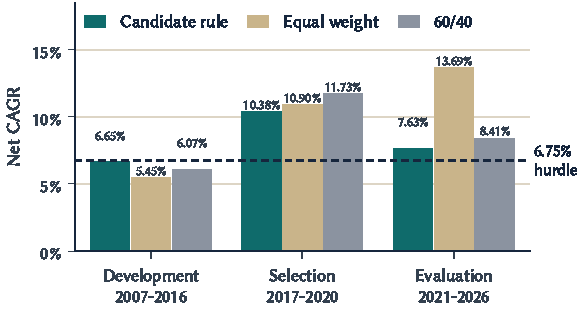
\includegraphics[width=\linewidth]{generated/figures/funding.pdf}
\end{minipage}

\noindent
\begin{minipage}[t]{0.47\textwidth}\vspace{0pt}
\subsection{Crisis replay of today's target}
{\begin{tabular}{@{}lrrr@{}}
\toprule
 & Endpoint & Drawdown & 60/40 DD \\
\midrule
GFC 2007--09 & \qeGfcReturn & \qeGfcDrawdown & \qeGfcDrawdownSixty \\
COVID-19 2020 & \qeCovidReturn & \qeCovidDrawdown & \qeCovidDrawdownSixty \\
Rate shock 2022 & \qeRatesReturn & \qeRatesDrawdown & \qeRatesDrawdownSixty \\
\bottomrule
\end{tabular}}
\qenote{Buy-and-hold ex-post replays, not the strategy's historical record. GFC drawdown exceeds the \qeBudgetDrawdown{} review line.}
\end{minipage}\hfill
\begin{minipage}[t]{0.50\textwidth}\vspace{0pt}
\subsection{Model validation}
{\begin{tabular}{@{}lrl@{}}
\toprule
99\% VaR, prior 500 days & Exceptions & Result \\
\midrule
Historical, last 250 & \qeBaselHs & \qezone{\qeBaselHsZone} \\
Normal, last 250 & \qeBaselNormal & \qezone{\qeBaselNormalZone} \\
Historical, 2021--26 & \qeHsEvalExceptions{} / \qeEvalSessions & Not rejected \\
Historical, full & \qeHsFullExceptions{} / \qeFullSessions & \textcolor{qered}{\sffamily\bfseries Rejected} \\
\bottomrule
\end{tabular}}
\qenote{Basel zones are educational. Non-rejection is not proof of safety.}
\end{minipage}

\subsection{What needs adjusting}
\begin{itemize}[itemsep=1pt]
\item \textbf{Funding.} Ending cash yield of \qeIncomeYield{} is below \qeSpending{} spending, so planned sales and liquidity need approval.
\item \textbf{Concentration.} XLE is \qeWeightXle{} of target but \qeShareXle{} of ES; GLD is \qeShareGld{}. Weight is not the same as risk.
\item \textbf{Drift.} Holdings passed a target cap on \qeDriftSessions{} of \qeActiveSessions{} sessions, peaking at \qeDriftMax{} in \qeDriftTicker{}. Targets are controlled; daily holdings are not.
\item \textbf{Monitoring.} Review quarterly. Escalate if ES 99\% exceeds \qeBudgetEs{}, drawdown exceeds \qeBudgetDrawdown{}, holdings pass a target cap, or exceptions cluster. Limits are not raised to make the portfolio pass.
\end{itemize}

\qenote{Rule: 504 prior sessions, monthly long-only minimum variance; each ETF at most 40\%, equities at most 35\%; 5 bp per unit traded. Day-level RF and ex-post CPI limits apply. AI materially assisted this work; independent human validation is pending and no university committee has approved it.}
\end{document}
